\documentclass[a4paper, 12pt]{article}

%Русский язык
\renewcommand{\familydefault}{\sfdefault}%шрифт
\usepackage[T2A]{fontenc} %кодировка
\usepackage[utf8]{inputenc} %кодировка исходного кода
\usepackage[english,russian]{babel} %локализация и переносы
%отступы 
\usepackage[left=2cm,right=2cm,top=2cm,bottom=3cm,bindingoffset=0cm]{geometry}
\usepackage{indentfirst}
%Вставка картинок
\usepackage{graphicx}
\graphicspath{}
\DeclareGraphicsExtensions{.pdf,.png,.jpg, .jpeg}

%Таблицы
\usepackage[table,xcdraw]{xcolor}
\usepackage{booktabs}

% Cсылки
\usepackage{hyperref}
\bibliographystyle{unsrt}
%Математика
\usepackage{physics}
\usepackage{amssymb, amsmath}

\DeclareMathOperator*{\sign}{sign}
\DeclareMathOperator*{\Real}{Re}
\DeclareMathOperator*{\Imag}{Im}
\DeclareMathOperator*{\arcsh}{arcsh}
\newcommand{\groupn}{\mathbb{Z}_n}

%%Окружение для многострочных уравнений
\usepackage{empheq}
\newenvironment{eqw}{\begin{equation} \begin{aligned}}   
    {\end{aligned}    \end{equation}}
\newenvironment{eqw*}{\begin{equation*} \begin{aligned}}   
    {\end{aligned}    \end{equation*}}
    
%Заголовок
\author{Нугманов Булат}
\title{Quasiprobability distributions of bright ‘‘banana’’ states}
\begin{document}
\maketitle
\section*{Вступление}
\begin{eqw}\label{Hamiltonian}
    \hat H_{Kerr} = \hbar \omega_0 \hat n + \hbar\gamma \hat n(\hat n - 1)
\end{eqw}
С точностью до переопределения $\omega_0$ можно интерпретировать гамильтониан следующим образом: пролетая через кристалл, каждая пара фотонов взаимодействует с энергией $\hbar\gamma / 2$.

В представлении вращающейся волны:
\begin{eqw}\label{Psi definition}
    \ket{\psi} = e^{-\frac{i}{\hbar}\hat H_{Kerr}\tau}\ket{\alpha} = e^{-\frac{\abs{\alpha}^2}{2}}\sum\limits_{n=0}^{\infty}\frac{\alpha^n}{\sqrt{n!}}e^{-i\Gamma n(n-1)}\ket{n},
\end{eqw}
где $\Gamma = \gamma \tau$ --- эффективный параметр нелинейности.

Функцию Хусими ранее считали по формулам из \cite{milburn1986quantum}, которые естественным образом следуют из определения функции Хусими:
\begin{eqw}\label{Husimi by def}
    Q(\beta) = \frac{\abs{\braket{\beta}{\psi}}^2}{\pi} = \frac{e^{-\abs{\alpha}^2-\abs{\beta}^2}}{\pi}\left|
	\sum\limits_{n = 0}^{\infty}\dfrac{\left(\alpha \beta^*\right)^n e^{-i \Gamma n(n-1)}}{n!}\right|^2
\end{eqw}

Как можно видеть из формулы \ref{Psi definition}, эволюция в Керровском гамильтониане не меняет распределения числа фотонов. Это значит, что при больших $\abs{\alpha}$ наиболее содержательная часть квазивероятностных распределений, так же как и у когерентного состояния будет достигаться при $\abs{\beta}\sim\abs{\alpha} \pm O(1)$.
% Это можно расписать более подробно. Что типо ширина гауссова профиля это 3 сигмы. Ну и для функций Хусими это 3, а для функций Вигнера 3/\sqrt{2}
Функцию Вигнера ранее считали двумя основными способами: численным решением дифференциального уравнения на эволюцию функции Вигнера во времени или прямым вычислением в каждой точке. Как показывают результаты \cite{stobinska2008wigner}, известные формулы для прямого вычисления оказываются неприменимыми для больших $\abs{\alpha}$. Они достаточно быстро приводят к переполнению и требуют около $O(\abs{\alpha}^4)$ слагаемых. Вычисление функции Вигнера с помощью численного решения уравнения в частных производных так же нельзя назвать быстрым, так как требуется большое количество точек на сетке.
\section*{Функция Хусими}
Слагаемые в суммировании по формуле \ref{Husimi by def} имеют пуассоновское распределение. При $\abs{\beta}\sim\abs{\alpha}\gg 1$ пуассоновское распределение вырождается в нормальное, так что пользуясь правилом 3-сигма мы получаем, что для достаточно точного вычисления функции Хусими требуется $\sim O(\abs{\alpha})$ слагаемых. (Для избежания переполнения, необходимо воспользоваться формулой Стирлинга для оценки $n!$) В данном разделе мы выведем формулу, которая выдаёт значения функции Хусими за $O(1)$ при $\abs{\alpha\beta}\gg1$ и $\abs{\Gamma}\ll 1$. 

Сначала заметим, что величины $\alpha$ и $\beta$ входят ряд для функции Хусими только вместе в конструкции $\alpha\beta^*$. Это несколько упрощает вычисления, потому что мы можем свести зависимость от трёх параметров ($\alpha,\;\beta,\;\Gamma$) к  зависимости лишь от двух ($\alpha\beta^*,\;\Gamma$). Введём для этого функцию $F$, через которую выражается функция Хусими:
\begin{subequations}
\renewcommand{\theequation}{\theparentequation.\arabic{equation}}
\begin{empheq}[]{align}\label{QtoF}
    &Q(\beta) = \frac{e^{-\abs{\alpha}^2-\abs{\beta}^2}}{\pi}\abs{F\left(\alpha\beta^*e^{i\Gamma}, e^{-i\Gamma}\right)}^2\\
    &F(A, e^{i\Gamma}) = \sum\limits_{n=0}^{\infty} \frac{A^n}{n!}e^{i\Gamma n^2}
\end{empheq}
\end{subequations}

При помощи интеграла гауссова типа мы сможем избавится от неудобного для аналитических вычислений множителя вида $e^{i\Gamma n^2}$:
\begin{subequations}
\renewcommand{\theequation}{\theparentequation.\arabic{equation}}
\begin{empheq}[]{align}
    \exp\left(i\Gamma n^2\right) = \frac{e^{i\frac{\pi}{4}\sign \Gamma}}{2\sqrt{\pi|\Gamma|}}
    &\int\limits_{-\infty}^{\infty} \exp\left(-\frac{i z^2}{4\Gamma} + i n z\right) dz\\
    F(A, e^{i\Gamma})=\sum\limits_{n=0}^{\infty} \frac{A^n e^{i\Gamma n^2}}{n!} = \frac{e^{i\frac{\pi}{4}\sign \Gamma}}{2\sqrt{\pi|\Gamma|}}
    &\int\limits_{-\infty}^{\infty} \exp\left(-\frac{i z^2}{4\Gamma} +  A e^{iz}\right) dz
\end{empheq}
\end{subequations}

К последнему выражению можно применить комплексный метод перевала. Для упрощения выражений сделаем некоторые переобозначения:
\begin{subequations}
\renewcommand{\theequation}{\theparentequation.\arabic{equation}}
\begin{empheq}[]{align}
    f(z) &=  \frac{z^2}{2i} + i Z e^{iz}\\
    Z &= -2i A \Gamma = R e^{i\Phi},\\
    F(A, e^{i\Gamma})&=\frac{e^{i\frac{\pi}{4}\sign \Gamma}}{2\sqrt{\pi|\Gamma|}}
    \int\limits_{-\infty}^{\infty}\exp\left(\frac{f(z)}{2\Gamma}\right)dz \label{integral row}
\end{empheq}
\end{subequations}
В нашем случае количество точек перевала $z_k$ бесконечно ($k\in\mathbb{Z}$). Их можно пронумеровать в соответствии номерами ветвей $W$-функции Ламберта:
\begin{eqw}\label{z_k def}
     f'(z_k) =0 \Rightarrow i Z e^{i z_k} = z_k \Rightarrow   z_k = i W_k(Z)
\end{eqw}
Схематичное положение перевальных точек $z_k$ и кривые постоянной фазы $\gamma_k$ через них отмечены на изображении \ref{saddle_points}. Отметим, что через каждое $z_k$ проходит две кривые постоянной фазы: одна из них соотвествует кривой наискорейшего спуска при $\Gamma > 0$, а другая при $\Gamma < 0$.

\begin{figure}
    \centering
    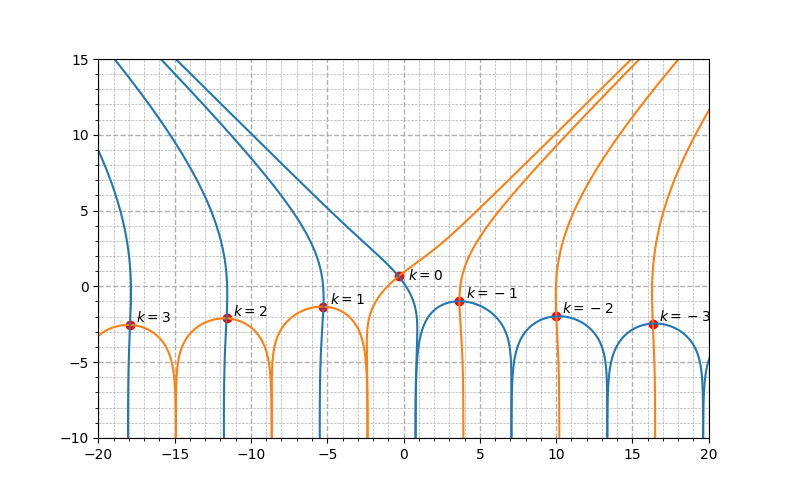
\includegraphics[width=0.75\textwidth]{v.png}
    \caption{Кривые постоянной фазы для интеграла \ref{integral row} при $Z=1+i$. Синим указаны кривые наискорейшего спуска $\gamma_k$ при $\Gamma < 0$, оранжевым --- при $\Gamma > 0$. Красные точки пересечения кривых --- точки перевала $f'(z_k)=0$.}\label{saddle_points}
\end{figure}

Детальное рассмотрение того, как деформировать контур интегрирования и учёт остаточных членов по формуле CFWW можно посмотреть в математическом приложении. Короче говоря, деформированный контур проходит лишь через половину всех $z_k$, что приводит нас к следующему результату:
\begin{eqw}\label{sum_k}
    \int\limits_{-\infty}^{\infty}\exp\left(\frac{f(z)}{2\Gamma}\right)dz = \sum\limits_{k=0}^{-\sign\Gamma \cdot \infty} \sqrt{\frac{4\Gamma}{{-i-z_k}}}\exp\left(\frac{ f(z_k)}{2\Gamma} \right)\left(1+O(\Gamma^2)\right)
\end{eqw}
Ключевой идеей дальнейшего рассуждения является замечание того факта, что $\abs{\exp\left(\frac{ f(z_k)}{2\Gamma} \right)}$ как функция $k$ имеет очень узкий гауссов профиль. Это значит, из всей суммы в уравнении \ref{sum_k} мы можем учитывать лишь $1$ или $2$ слагаемых, вносящих наибольший вклад. В большинстве случаев достаточно учитывать лишь одно слагаемое под номером $\bar{k}$, что можно увидеть на рисунке \ref{where_best_k_bar2}. Вывод ограничений на применимость таких рассуждений, нахождение оптимального $\bar{k}(Z)$ и поведение лидирующего вклада как функцию $\Phi=\arg Z$ можно посмотреть в математическом приложении. 
\begin{figure}
    \centering
    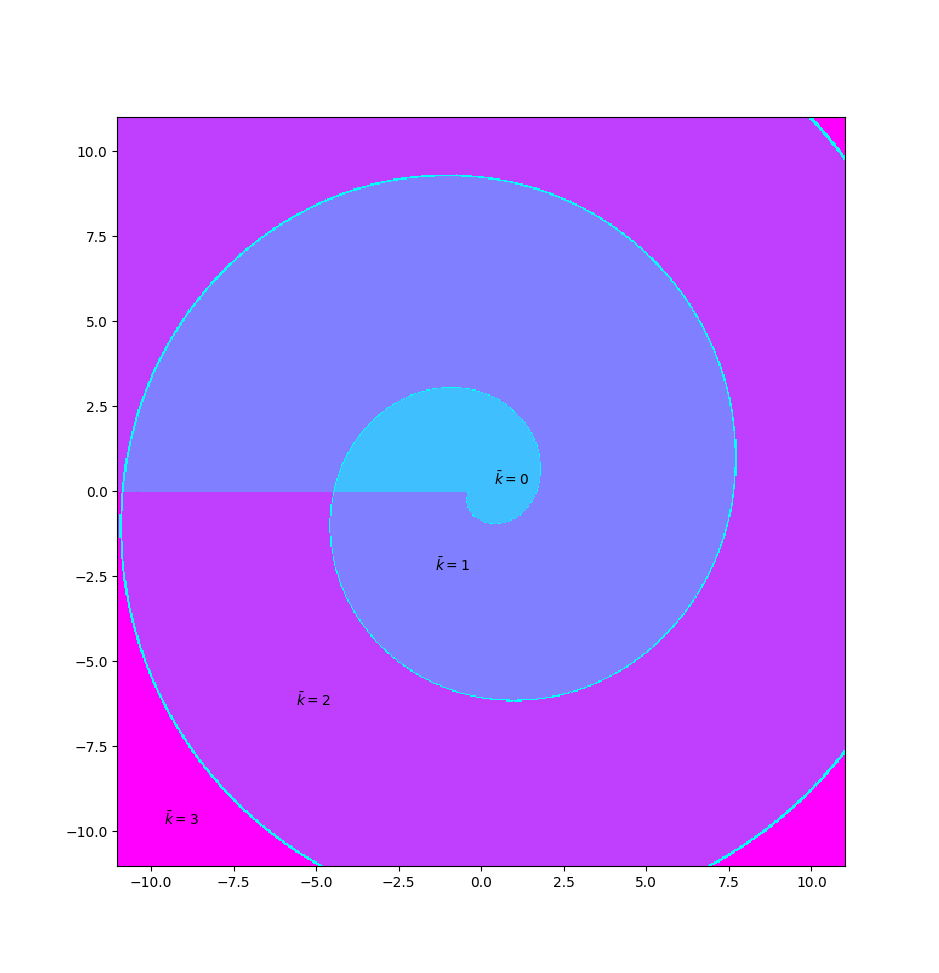
\includegraphics[width=0.75\textwidth]{where_best_k_bar2.png}
    \caption{На комплексной плоскости для каждой точки $Z$ отмечены $\bar{k}$, вносящие основной вклад в сумму \ref{sum_k}. Узкая голубая линия означает то небольшое множество точек, в которых $\abs{\Real f(z_k) - \Real f(z_{k+1})}<2\Gamma$. На графике изображена картинка при $\Gamma=0.01$. При уменьшении $\Gamma$ мера точек $Z$ при которых в сумме \ref{sum_k} необходимо учитывать 2 слагаемых ($\bar{k}$ и $\bar{k}+1$) снижается.}\label{where_best_k_bar2}
\end{figure}

Собирая воедино выражения \ref{z_k def}, \ref{sum_k}, \ref{integral row} и \ref{QtoF} мы приходим к следующему выражению:
\begin{eqw}\label{Qgood}
    \text{Большое выражение}
\end{eqw}
\section*{Функция Вигнера}
Основной идеей для поиска значений функции Вигнера является её связь с функцией Хусими через характеристические функции $C_{s, a}$ или преобразование Фурье $\mathcal{F}$ \textcolor{red}{(нужна ссылка)}:
\begin{eqw}\label{FourierC}
    C_s(z) = \mathcal{F}\left\{W\right\}(z) = e^{\frac{\abs{z}^2}{2}} \mathcal{F}\left\{Q\right\}(z) = e^{\frac{\abs{z}^2}{2}} C_a(z)
\end{eqw}
Мы не можем воспользоваться уже известным нам приближением для функции Хусими \ref{Qgood} и численным расчётом преобразований Фурье, так как в формуле фигурирует экспоненциальное завышение частот $e^{\frac{\abs{z}^2}{2}}$. Подстановка функции Хусими в форме \ref{Husimi by def} представляется весьма затруднительной, поэтому мы предлагаем другую форму записи для функции $F$ \ref{QtoF}, через которую выражается функция Хусими.
Кто-то может заметить, что при $\frac{\Gamma}{2\pi} = \frac{k}{n}\in\mathbb{Q}$ для функции $F$ можно найти замкнутое выражение с конечным числом слагаемых: 
\begin{eqw}\label{Fexp}
    F(A, e^{i\Gamma}) = \frac{\sum_{j\in\groupn}\exp\left(-i\Gamma j^2 + A e^{2ij\Gamma}\right)}{\sum_{j\in\groupn}\exp\left(-i\Gamma j^2\right)}
\end{eqw}

Одно из возможных доказательств через функционально-дифференциальное уравнение на функцию $F$ можно найти математическом приложении. Представление \ref{Fexp} в совокупности с \ref{QtoF} является гораздо более удобной формой, так как оно сводит нахождение преобразований Фурье  \ref{FourierC} к простому вычислению интегралов гауссова типа. Результатом громоздких выкладок, представленных в математическом приложении, является следующая формула, которая справедлива при произвольных $\Gamma\in\mathbb{R}$:
\begin{subequations}\label{Q to W for banan}
\renewcommand{\theequation}{\theparentequation.\arabic{equation}}
\begin{empheq}[]{align}
    W(\beta) &= \frac{2}{\pi}e^{\abs{\alpha}^2 - 2\left(\abs{\alpha} - \abs{\beta}\right)^2}\sum\limits_{m=0}^{\infty} \frac{\left(-|\alpha|^2\right)^m}{m!}\left|F(2\alpha \beta^* e^{i\Gamma(2m-1)}, e^{i\Gamma})e^{-2\abs{\alpha\beta^*}}\right|^2\label{W too big exp}\\
    W(\beta) &= 2e^{2|\beta|^2}\sum\limits_{m=0}^{\infty} \frac{\left(-|\alpha|^2\right)^m}{m!}Q(2\beta e^{-i\Gamma 2m})
\end{empheq}
\end{subequations}


Однако данная форма также не применима для численных расчётов. При $\abs{\beta}\sim\abs{\alpha}$, суммируя величины порядка $\exp\left(\abs{\alpha}^2\right)$ в формуле \ref{W too big exp} мы должны достичь точности порядка $\exp\left(-\abs{\alpha}^2\right)$, что представляется невозможным при больших $\abs{\alpha}$. Наконец, разложим выражение \ref{Q to W for banan} в ряд Фурье по $\arg{\beta}$:
\begin{eqw}\label{Fourier W}
    \Phi_0 &= \arg\left(\alpha\beta^* e^{2i\Gamma}\right)\\
     W(\beta) &= \frac{2}{\pi}e^{-2\left(\abs{\beta} - \abs{\alpha}\right)^2}
     \sum\limits_{k=-\infty}^{+\infty} e^{ik\Phi_0} I_{k}\left(4\abs{\alpha\beta^*}e^{-i\Gamma k}\right)
     \exp\left(\abs{\alpha}^2 (1-e^{-2ik\Gamma})-4\abs{\alpha\beta^*}\right)
\end{eqw}
В последнем выражении можно использовать асимптотику для модифицированной функции Бесселя $I_k$, которая будет работать как при малых, так и при больших $k$. Пользуясь выражением из \cite{bateman1953higher} при $k\Gamma\in\left(-\frac{\pi}{2}, \frac{\pi}{2}\right)$ приходим к удобо считаемому выражению для функции Вигнера:
\begin{eqw}\label{W final}
    &W(\beta) \approx \frac{1}{\pi}\sqrt{\frac{2}{\pi}}\sum\limits_{k=-\infty}^{+\infty} \left(\left(4\abs{\alpha\beta^*}e^{-ik\Gamma}\right)^2+k^2\right)^{-\frac{1}{4}}\exp\left(-2\left(\abs{\beta} - \abs{\alpha}\right)^2 + ik\Phi_0 + \right.\\
    &+\left.
    \abs{\alpha}^2\left(1-e^{-2ik\Gamma}\right)-4\abs{\alpha\beta^*}+
    \sqrt{\left(4\abs{\alpha\beta^*}e^{-ik\Gamma}\right)^2+k^2}-k\arcsh\left(\frac{k}{4\abs{\alpha\beta^*}e^{-ik\Gamma}}\right)\right)
\end{eqw}
Более подробно о разложении в ряд Фурье \ref{Fourier W}, об условиях применимости и остаточных членах разложения \ref{W final} можно прочитать в математическом приложении.
\section*{Заключение}
Перечислим основные результаты данной статьи. Мы научились считать квазивероятностные функции Хусими и Вигнера яркого бананового состояния. Предложенные алгоритмы позволяют посчитать функцию Хусими за $O(1)$ и функцию Вигнера за $O(\abs{\alpha})$ при $\Gamma\sim\abs{\alpha}^{-2}\ll1$. Программная реализация доступна на гитхабе \cite{mygit}.
\nocite{*}
\bibliography{references}
\end{document}